\documentclass[a4paper,showframe,11pt]{report}\usepackage[]{graphicx}\usepackage[]{color}
%% maxwidth is the original width if it is less than linewidth
%% otherwise use linewidth (to make sure the graphics do not exceed the margin)
\makeatletter
\def\maxwidth{ %
  \ifdim\Gin@nat@width>\linewidth
    \linewidth
  \else
    \Gin@nat@width
  \fi
}
\makeatother

\definecolor{fgcolor}{rgb}{0.196, 0.196, 0.196}
\newcommand{\hlnum}[1]{\textcolor[rgb]{0.063,0.58,0.627}{#1}}%
\newcommand{\hlstr}[1]{\textcolor[rgb]{0.063,0.58,0.627}{#1}}%
\newcommand{\hlcom}[1]{\textcolor[rgb]{0.588,0.588,0.588}{#1}}%
\newcommand{\hlopt}[1]{\textcolor[rgb]{0.196,0.196,0.196}{#1}}%
\newcommand{\hlstd}[1]{\textcolor[rgb]{0.196,0.196,0.196}{#1}}%
\newcommand{\hlkwa}[1]{\textcolor[rgb]{0.231,0.416,0.784}{#1}}%
\newcommand{\hlkwb}[1]{\textcolor[rgb]{0.627,0,0.314}{#1}}%
\newcommand{\hlkwc}[1]{\textcolor[rgb]{0,0.631,0.314}{#1}}%
\newcommand{\hlkwd}[1]{\textcolor[rgb]{0.78,0.227,0.412}{#1}}%
\let\hlipl\hlkwb

\usepackage{framed}
\makeatletter
\newenvironment{kframe}{%
 \def\at@end@of@kframe{}%
 \ifinner\ifhmode%
  \def\at@end@of@kframe{\end{minipage}}%
  \begin{minipage}{\columnwidth}%
 \fi\fi%
 \def\FrameCommand##1{\hskip\@totalleftmargin \hskip-\fboxsep
 \colorbox{shadecolor}{##1}\hskip-\fboxsep
     % There is no \\@totalrightmargin, so:
     \hskip-\linewidth \hskip-\@totalleftmargin \hskip\columnwidth}%
 \MakeFramed {\advance\hsize-\width
   \@totalleftmargin\z@ \linewidth\hsize
   \@setminipage}}%
 {\par\unskip\endMakeFramed%
 \at@end@of@kframe}
\makeatother

\definecolor{shadecolor}{rgb}{.97, .97, .97}
\definecolor{messagecolor}{rgb}{0, 0, 0}
\definecolor{warningcolor}{rgb}{1, 0, 1}
\definecolor{errorcolor}{rgb}{1, 0, 0}
\newenvironment{knitrout}{}{} % an empty environment to be redefined in TeX

\usepackage{alltt}
\usepackage{standalone}
\standalonetrue
\ifstandalone
  \usepackage{../../haziq_thesis}
  \usepackage{../../haziq_maths}
  \usepackage{../../haziq_glossary}
  \addbibresource{../../bib/haziq.bib}
  \externaldocument{../01/.texpadtmp/introduction}
\fi




\IfFileExists{upquote.sty}{\usepackage{upquote}}{}
\begin{document}

Let's look at some toy examples to illustrate classification using I-probit models. First is a binary classification task based on two predictors. This data set consists of 300 points from two spirals with some Gaussian noise added. A plot is shown below.

\begin{knitrout}
\definecolor{shadecolor}{rgb}{1, 1, 1}\color{fgcolor}\begin{kframe}
\begin{alltt}
\hlstd{R> }\hlstd{spiral} \hlkwb{<-} \hlkwd{gen_spiral}\hlstd{(}\hlkwc{n} \hlstd{=} \hlnum{300}\hlstd{,} \hlkwc{sd} \hlstd{=} \hlnum{0.07}\hlstd{)}
\hlstd{R> }\hlkwd{plot}\hlstd{(spiral)}
\end{alltt}
\end{kframe}\begin{figure}[h]

{\centering 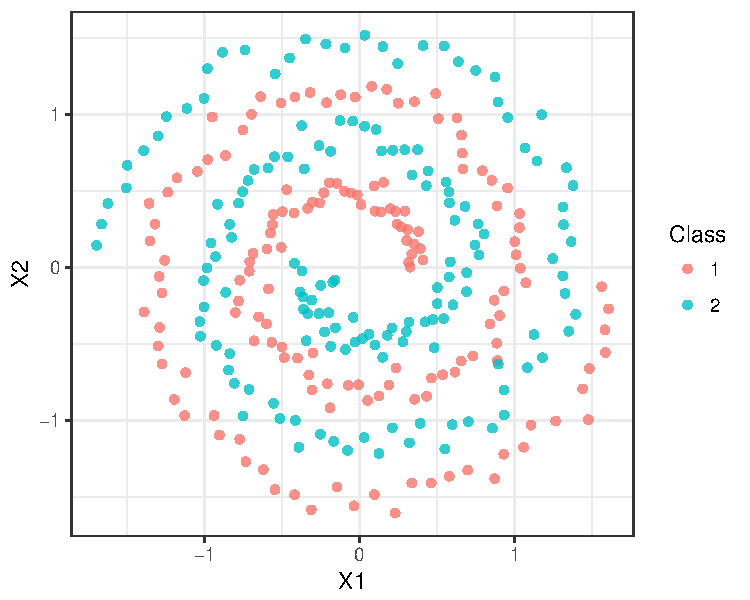
\includegraphics[width=0.7\linewidth]{figure/spiral_data-1} 

}

\caption[Spiral data set]{Spiral data set.}\label{fig:spiral_data}
\end{figure}


\end{knitrout}

We tried a few models. First with the linear canonical kernel. This gave very poor results (training error rate of 50\% is basically just guess-work). Not surprising because the problem hardly seems linear in nature. Best to go with a smooth function, so we tried the fBm kernel. This gave an improved training error rate (31.3\%) but judging by the predictive plot, there still is room for improvement.

\begin{knitrout}
\definecolor{shadecolor}{rgb}{1, 1, 1}\color{fgcolor}\begin{kframe}
\begin{alltt}
\hlstd{R> }\hlcom{# Bad results, linear functions not able to predict spirals well}
\hlstd{R> }\hlstd{(mod1} \hlkwb{<-} \hlkwd{iprobit}\hlstd{(y} \hlopt{~} \hlstd{X1} \hlopt{+} \hlstd{X2, spiral,} \hlkwc{kernel} \hlstd{=} \hlstr{"Canonical"}\hlstd{))}
\end{alltt}
\begin{verbatim}
## ===========
## Converged after 15 iterations.
## Training error rate: 50.00 %
## Lower bound value: -214.0725 
## 
##     alpha lambda[1] lambda[2] 
##   0.00004   0.00000   2.88634
\end{verbatim}
\begin{alltt}
\hlstd{R> }\hlkwd{iplot_predict}\hlstd{(mod1)}
\end{alltt}
\end{kframe}\begin{figure}[h]

{\centering 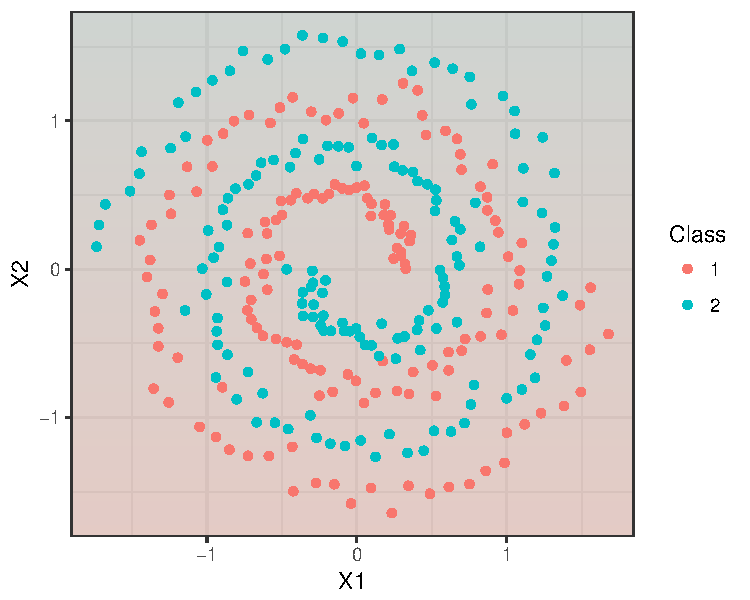
\includegraphics[width=0.7\linewidth]{figure/spiral_canonical-1} 

}

\caption[Canonical kernel with multiple scale parameters]{Canonical kernel with multiple scale parameters.}\label{fig:spiral_canonical}
\end{figure}


\end{knitrout}

\begin{knitrout}
\definecolor{shadecolor}{rgb}{1, 1, 1}\color{fgcolor}\begin{kframe}
\begin{alltt}
\hlstd{R> }\hlcom{# Getting there, but still not nice}
\hlstd{R> }\hlstd{(mod2} \hlkwb{<-} \hlkwd{iprobit}\hlstd{(y} \hlopt{~} \hlstd{X1} \hlopt{+} \hlstd{X2, spiral,} \hlkwc{kernel} \hlstd{=} \hlstr{"FBM"}\hlstd{))}
\end{alltt}
\begin{verbatim}
## ======================================================================
## Convergence criterion not met.
## Training error rate: 31.33 %
## Lower bound value: -204.2227 
## 
##     alpha lambda[1] lambda[2] 
##   0.00484  -0.00263   1.26369
\end{verbatim}
\begin{alltt}
\hlstd{R> }\hlkwd{iplot_predict}\hlstd{(mod2)}
\end{alltt}
\end{kframe}\begin{figure}[h]

{\centering 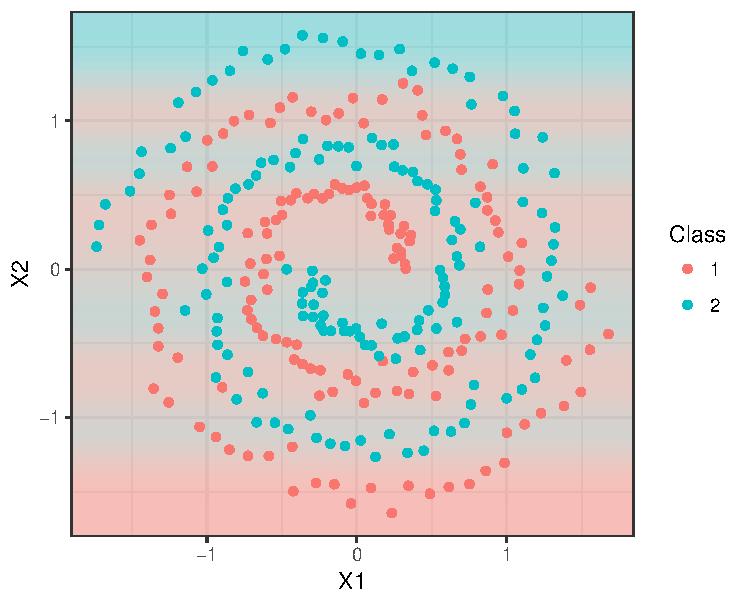
\includegraphics[width=0.7\linewidth]{figure/spiral_fbm-1} 

}

\caption[fBm kernel with multiple scale parameters]{fBm kernel with multiple scale parameters.}\label{fig:spiral_fbm}
\end{figure}


\end{knitrout}

\begin{knitrout}
\definecolor{shadecolor}{rgb}{1, 1, 1}\color{fgcolor}\begin{kframe}
\begin{alltt}
\hlstd{R> }\hlcom{# Turns out the scale parameters matter here}
\hlstd{R> }\hlstd{(mod3} \hlkwb{<-} \hlkwd{iprobit}\hlstd{(y} \hlopt{~} \hlstd{X1} \hlopt{+} \hlstd{X2, spiral,} \hlkwc{kernel} \hlstd{=} \hlstr{"FBM"}\hlstd{,} \hlkwc{one.lam} \hlstd{=} \hlnum{TRUE}\hlstd{))}
\end{alltt}
\begin{verbatim}
## ==========================================================
## Converged after 82 iterations.
## Training error rate: 1.67 %
## Lower bound value: -162.9976 
## 
##   alpha  lambda 
## 0.00497 5.16273
\end{verbatim}
\begin{alltt}
\hlstd{R> }\hlkwd{iplot_predict}\hlstd{(mod3)}
\end{alltt}
\end{kframe}\begin{figure}[h]

{\centering 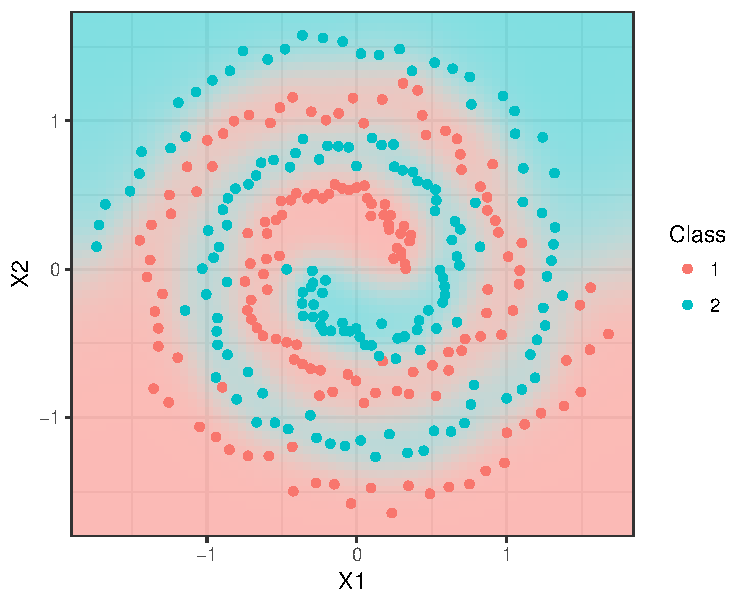
\includegraphics[width=0.7\linewidth]{figure/spiral_fbm_onelam-1} 

}

\caption[fBm kernel with a single shared scale parameter]{fBm kernel with a single shared scale parameter.}\label{fig:spiral_fbm_onelam}
\end{figure}


\end{knitrout}

It turns out that retstricting the model to have a single scale parameter works best, coupled with the fBm kernel. This seems to suggest that the two variables are similarly scaled and effects the latent response in a similar magnitude. Indeed, the $X_1$ and $X_2$ variables are quite similar in that they are points from two spirals mirroring each other. We are able to get a training error rate of 1.67\%, and incidentally this model gives the highest lower-bound value as well.

One thing that was noticed with this data set was that different starting values led to possibly different converged parameter estimates. This leads us to believe that the variational lower bound to be maximised has multiple local optima. One way to overcome this is to perform multiple restarts and keep the results from the highest lower bound value. This is something to look out for when analysing real-data examples.

The next example is a four-class classification data set that is meant to be linearly separable in two dimensions. Random noise was added to the $X_1$ and $X_2$ component from four equidistant points (representing four distinct classes) around a circle of radius three. 125 points were generated for each class, thereby giving a total of 500 data points altogether. Here is a plot of the data set.

\begin{knitrout}
\definecolor{shadecolor}{rgb}{1, 1, 1}\color{fgcolor}\begin{kframe}
\begin{alltt}
\hlstd{R> }\hlstd{mixture} \hlkwb{<-} \hlkwd{gen_mixture}\hlstd{(}\hlkwc{n} \hlstd{=} \hlnum{500}\hlstd{,} \hlkwc{m} \hlstd{=} \hlnum{4}\hlstd{,} \hlkwc{sd} \hlstd{=} \hlnum{1.5}\hlstd{)}
\hlstd{R> }\hlstd{(mod} \hlkwb{<-} \hlkwd{iprobit}\hlstd{(y} \hlopt{~} \hlstd{X1} \hlopt{+} \hlstd{X2, mixture))}
\end{alltt}
\begin{verbatim}
## ======================================================================
## Convergence criterion not met.
## Training error rate: 8.80 %
## Lower bound value: -194.2465 
## 
##            Class = 1 Class = 2 Class = 3 Class = 4
## alpha       -0.12285  -0.71550  -0.72534  -0.07966
## lambda[1,]   1.28355   0.00000   0.70112   0.00000
## lambda[2,]   0.00000   0.25543   0.00000   1.02738
\end{verbatim}
\end{kframe}
\end{knitrout}

We fit a canonical I-probit model, and get the following results.

\begin{knitrout}
\definecolor{shadecolor}{rgb}{1, 1, 1}\color{fgcolor}\begin{kframe}
\begin{alltt}
\hlstd{R> }\hlkwd{plot}\hlstd{(mixture)}
\hlstd{R> }\hlkwd{iplot_predict}\hlstd{(mod)}
\end{alltt}
\end{kframe}\begin{figure}[h]

{\centering 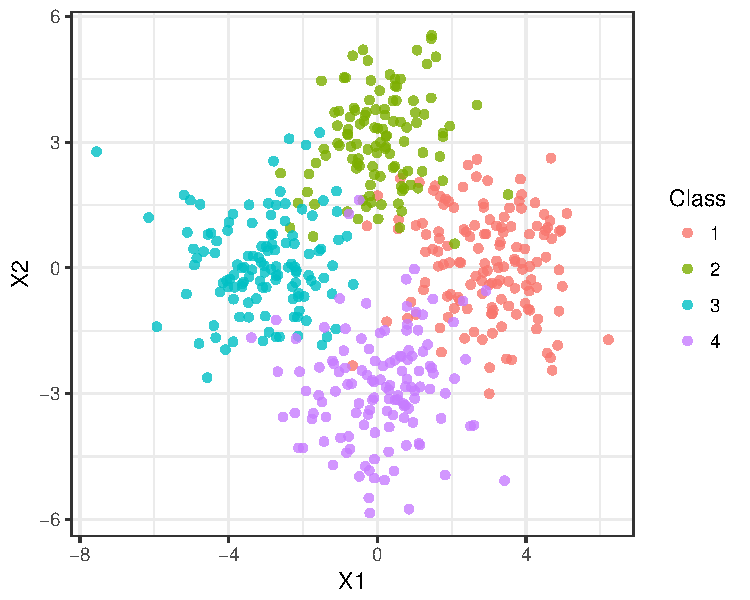
\includegraphics[width=0.49\linewidth]{figure/mixture_mod_plot-1} 
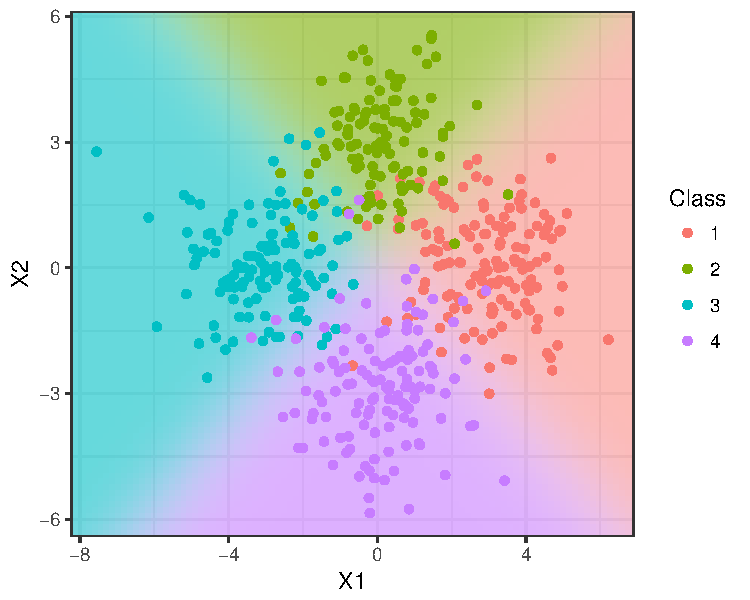
\includegraphics[width=0.49\linewidth]{figure/mixture_mod_plot-2} 

}

\caption[Canonical kernel is able to linearly separate the data points]{Canonical kernel is able to linearly separate the data points.}\label{fig:mixture_mod_plot}
\end{figure}


\end{knitrout}

\end{document}


